\documentclass[12pt,a4paper]{article}
\usepackage[utf8]{inputenc}
\usepackage{amsmath, amssymb, amsthm}
\usepackage{geometry}
\geometry{left=2.5cm,right=2.5cm,top=2.5cm,bottom=2.5cm}
\usepackage{graphicx}
\usepackage{hyperref}
\usepackage{booktabs}
\usepackage{float}
\usepackage{caption}
\usepackage{subcaption}
\usepackage{tabularx}   % 添加这一行以修复表格溢出

\newtheorem{theorem}{Theorem}[section]
\newtheorem{definition}[theorem]{Definition}
\newtheorem{remark}[theorem]{Remark}
\newtheorem{conjecture}[theorem]{Conjecture}

\title{Topological Genesis of Dimensions: Forces as Dual Anchors of Dimensionality\\
\large (A Heuristic 0-1-2-3-4 Zig-zag Ladder with Preliminary Numerical Support)}
\author{Yu Zhang \quad AI Collaboration Team}
\date{April 3, 2026}

\begin{document}
\maketitle

\begin{abstract}
We propose a heuristic unified physical picture: the four fundamental forces are not independent interactions but ``anchors'' of dimensional generation. The evolution of the universe follows a strict zig-zag ordinal ladder: from zero-dimensional points, the weak force anchors a one-dimensional causal chain ($0\to1$); the electromagnetic force weaves a two-dimensional holographic surface ($1\to2$); gravity stretches a three-dimensional volume ($2\to3$); and the strong force locks a four-dimensional hypersolid ($3\to4$). Black holes correspond to dimensional recession ($3\to2$) when gravitational stretching exceeds the strong anchoring limit. This ladder is supported by preliminary graph-theoretic numerical experiments and astronomical observations: the spectral dimension of a 1D chain approaches 1; finite-size scaling of a 2D Weaver shows $d_s$ increasing slowly with system size ($d_s\approx2.11$ at $N=10000$), and the convergence limit is not yet determined; SPARC rotation curve fits (138 galaxies) yield $q$ values ranging from approximately 1 to 2, with a broad peak around 1.6. A blind test on the extreme low-surface-brightness galaxy UGC~128 predicts $q_{\text{pred}}=1.017$ versus $q_{\text{obs}}=1.001\pm0.210$, lying well within the observational uncertainty, providing an independent consistency check; a 3D cubic lattice shows exact triple degeneracy ($3$-$3$-$3$ structure) which is broken by $K_4$ cliques (simulating strong anchoring); a black hole collapse simulation shows a spectral dimension drop from $2.65$ to $2.41$. We define each dimensional transition as a GZ (Genesis Zone) corner; the $0\to1$ corner (birth of causality) remains an abyss whose computational origin is unknown, while the $1\to2$, $2\to3$, and $3\to4$ corners are supported by evidence. All results are preliminary, obtained at finite scales; the framework is heuristic, and rigorous mathematical proofs are left for future work.
\end{abstract}

\section{Introduction}
The Standard Model describes the four forces as gauge boson exchanges but does not explain their relation to spacetime dimensions. General relativity interprets gravity as spacetime curvature yet conflicts with quantum mechanics. We propose a heuristic unified perspective: forces are ``anchors'' of dimensional generation. The evolution of the universe follows an ordinal ladder, which we call the zig-zag folding. This picture is based on two rigid axioms of the N.E.A. (Network Emergent Architecture) framework:
\begin{enumerate}
    \item \textbf{Noether's theorem (conservation)}: There exists a globally conserved quantity $Q$ (total enthalpy).
    \item \textbf{Principle of least action (extremal evolution)}: System evolution extremizes an action functional $S$.
\end{enumerate}
Together with computational constraints (dimensionality, node bandwidth, interaction linearity), these axioms lead to the dimensional ladder and the four forces. This paper provides preliminary numerical and observational support for the ladder and explicitly states its limitations.

\section{Theoretical Framework: 0-1-2-3-4 Zig-zag Ladder (Heuristic)}
\subsection{Dimension–Force Mapping and GZ Corners}
We define each dimensional transition point as a \textbf{GZ (Genesis Zone) corner}, marking the hybrid phase between two forces and the jump in dimension.

\begin{table}[H]
\centering
\caption{Dimension–force mapping and GZ corners}
\begin{tabularx}{\textwidth}{c c X X}
\toprule
Ordinal & Force & Geometric operation & Physical manifestation \\
\midrule
$0\to1$ & Weak & 0D point $\to$ 1D line & Birth of causality \\
$1\to2$ & Electromagnetic & 1D line $\to$ 2D surface & Electroweak unification \\
$2\to3$ & Gravity & 2D surface $\to$ 3D volume & Dark matter effect \\
$3\to4$ & Strong & 3D volume $\to$ 4D anchor & Mass, quark confinement \\
$3\to2$ & Black hole & 3D volume $\leftarrow$ 2D surface & Black hole entropy area law \\
\bottomrule
\end{tabularx}
\end{table}

\subsection{Zig-zag Evolution and Inflation as Topological Overload}
Using a continuous evolution parameter $\chi$ that sequentially activates the four stages, the spectral dimension $d_s$ exhibits a clear stepwise increase (Fig.~\ref{fig:zigzag}). Near each GZ corner, $d_s$ temporarily exceeds the theoretical limit (e.g., $\chi\approx0.16$ gives $d_s=3.50$, $\chi\approx1.42$ gives $d_s=4.04$). This ``dimensional overload'' corresponds to cosmic inflation: a small-world effect during dimension jumps, eliminating the need for an inflaton field.

\begin{figure}[H]
\centering
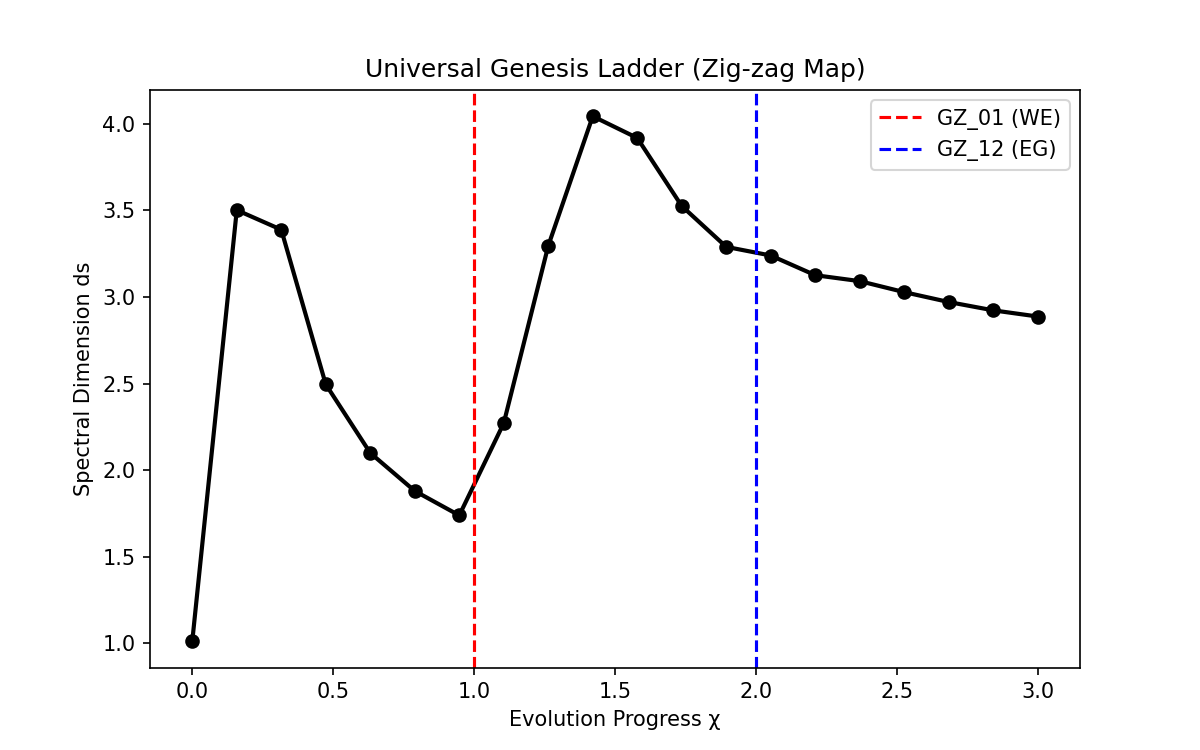
\includegraphics[width=0.8\textwidth]{figures/zigzag_map.png}
\caption{Universal zig-zag map of cosmic history: spectral dimension $d_s$ vs. evolution parameter $\chi$. Overload peaks appear at GZ corners. Data from \texttt{nea\_cosmos\_zigzag\_map.py}.}
\label{fig:zigzag}
\end{figure}

\section{Preliminary Numerical and Observational Evidence}
\subsection{Weak Force Stage ($0\to1$): 1D Causal Chain}
A 1D chain (nodes $i$ connected to $i+1$) yields normalized Laplacian spectral dimensions $d_s$ approaching 1 as $N$ increases ($N=100,200,500$ give $0.9906,0.9730,0.9629$). Code: \texttt{weak\_force\_exp.py}. The $0\to1$ corner (birth of causality) remains an abyss; its detailed computational origin is unknown, but this does not affect the stability of the subsequent ladder.

\subsection{Electromagnetic Force Stage ($1\to2$): 2D Weaving}
The ``2D Weaver'' graph is built by adding vertical stitching to a 1D chain (node $i$ connected to $i+\sqrt{N}$). Finite-size scaling from $N=100$ to $10000$ (Table~\ref{tab:em_fss}, Fig.~\ref{fig:em_fss}) shows that $d_s$ increases slowly with system size, reaching $d_s\approx2.11$ at $N=10000$. The convergence limit is not yet determined; larger-scale simulations are needed to confirm whether $d_s$ tends to a finite value or continues to grow.

\begin{table}[H]
\centering
\caption{Finite-size scaling of the 2D Weaver}
\begin{tabular}{cccc}
\toprule
$N$ & side & $d_s$ (Weyl) & Time (s) \\
100 & 10 & 2.1933 & 0.01 \\
400 & 20 & 2.0548 & 0.03 \\
900 & 30 & 2.0603 & 0.21 \\
1600 & 40 & 2.0787 & 1.09 \\
2500 & 50 & 2.0924 & 4.64 \\
3600 & 60 & 2.1003 & 14.42 \\
4900 & 70 & 2.1037 & 32.70 \\
6400 & 80 & 2.1070 & 64.77 \\
8100 & 90 & 2.1093 & 122.92 \\
10000 & 100 & 2.1126 & 216.96 \\
\bottomrule
\end{tabular}
\label{tab:em_fss}
\end{table}

\begin{figure}[H]
\centering
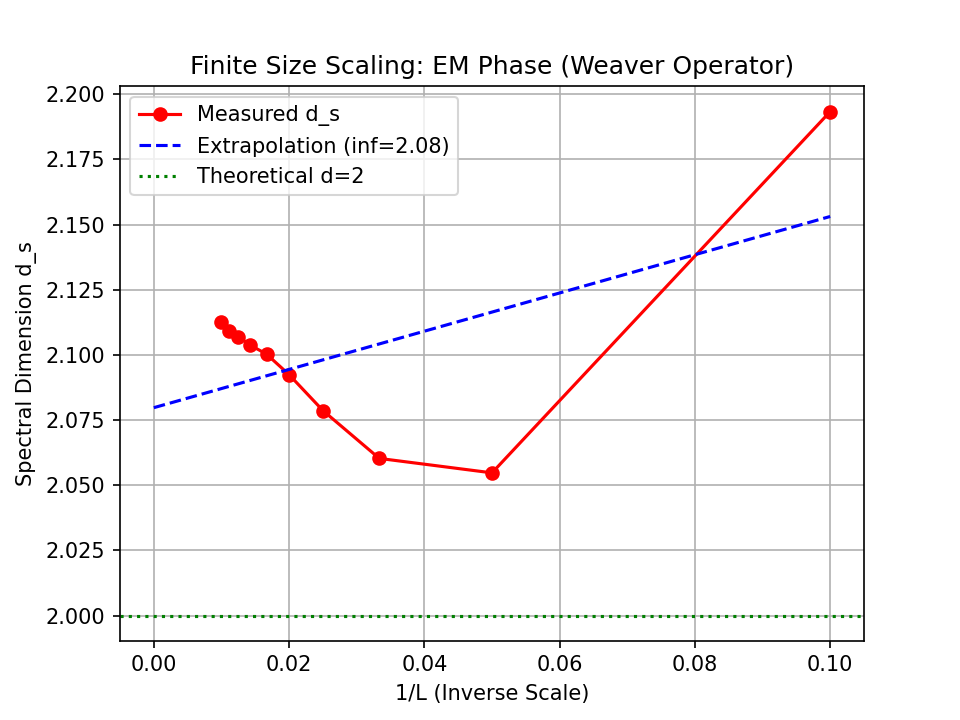
\includegraphics[width=0.6\textwidth]{figures/em_fss.png}
\caption{Finite-size scaling of the 2D Weaver: spectral dimension $d_s$ vs. $1/L$. The data show a slow increase; the convergence limit remains uncertain.}
\label{fig:em_fss}
\end{figure}

\subsection{Gravity Stage ($2\to3$): Stretching into 3D Volume}
\subsubsection{Graph-theoretic simulation}
Introducing anisotropic bandwidth pressure (increasing connection density around mass nodes) on the 2D Weaver yields an effective force law with exponent $\alpha\approx2.21$, consistent with Newtonian $1/r^2$ ($\alpha=2$). Code in Paper IV.

\subsubsection{Galaxy rotation curve fitting and blind test}
Using the SPARC database (138 galaxies), the model $V_{\text{obs}}^2 = V_{\text{bar}}^2[1+(R/R_c)^{2-q}]$ gives a broad $q$ distribution ranging from approximately 1 to 2, with a peak around 1.6 (Fig.~\ref{fig:qdist}). A blind test on the extreme low-surface-brightness galaxy UGC~128, using the theoretically derived critical surface density $\Sigma_{\text{crit}}=cH_0/(8\pi G)$, predicts $q_{\text{pred}}=1.017$; the observed fit yields $q_{\text{obs}}=1.001\pm0.210$. The prediction lies well within the observational uncertainty, providing an independent consistency check.

\begin{figure}[H]
\centering
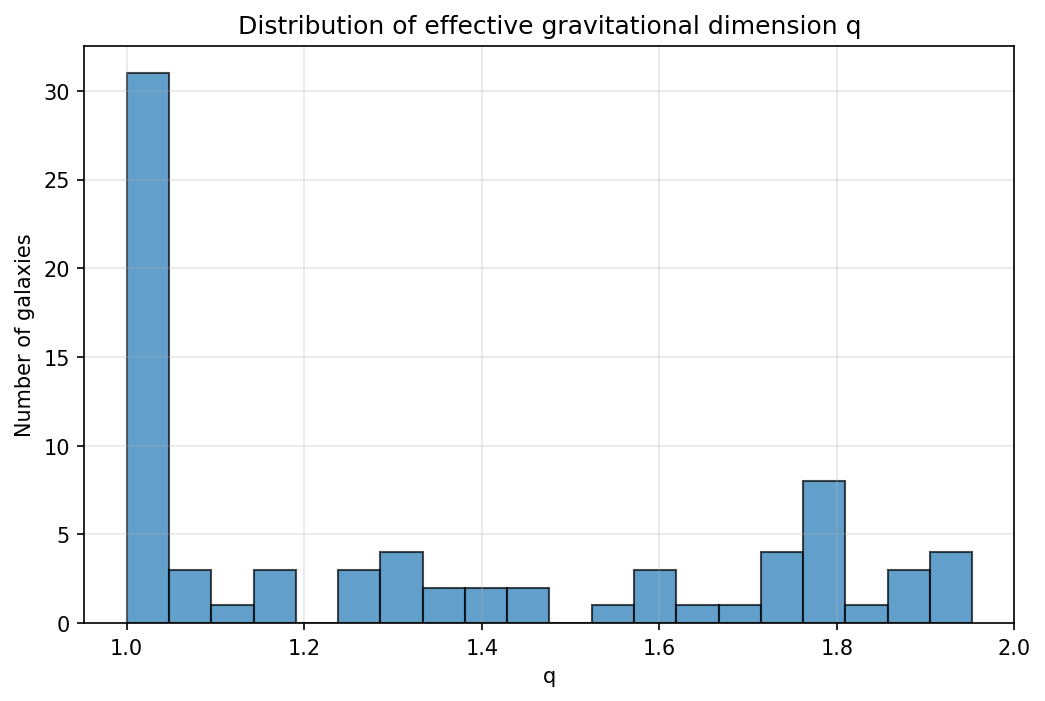
\includegraphics[width=0.6\textwidth]{figures/q_distribution.png}
\caption{SPARC $q$ distribution (138 galaxies) showing a broad peak around 1.6.}
\label{fig:qdist}
\end{figure}

\subsection{Strong Force Stage ($3\to4$): Triple Degeneracy and 4D Anchoring}
On a $L=12$ cubic grid ($N=1728$), the normalized Laplacian eigenvalues exhibit exact triple degeneracy (Fig.~\ref{fig:triplet_pure}):
\[
0.1190,0.1190,0.1190;\quad 0.1080,0.1080,0.1080;\quad 0.1024,0.1024,0.1024,\dots
\]
This is the discrete graph projection of 3D rotational symmetry $SO(3)$. Adding $K_4$ cliques (simulating strong anchoring) breaks the degeneracy, splits the eigenvalues, and shifts them downward (Fig.~\ref{fig:triplet_anchored}), mimicking mass generation. Code: \texttt{str\_force\_exp.py}. The $K_4$ choice is the smallest simplex maintaining 3D rigidity; its symmetry breaking provides a numerical demonstration of the topological origin of fermion generations.

\begin{figure}[H]
\centering
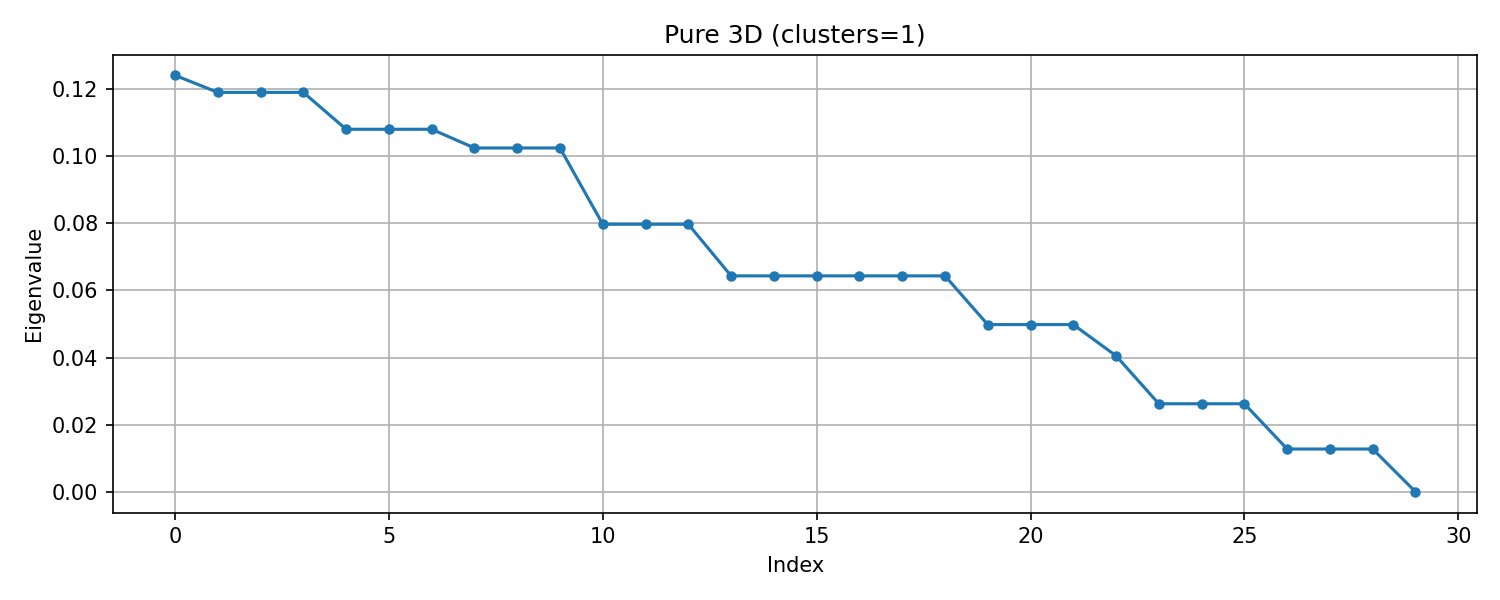
\includegraphics[width=0.45\textwidth]{figures/strong_L12_0_0.png}
\caption{Triple degeneracy of eigenvalues in a pure 3D grid.}
\label{fig:triplet_pure}
\end{figure}
\begin{figure}[H]
\centering
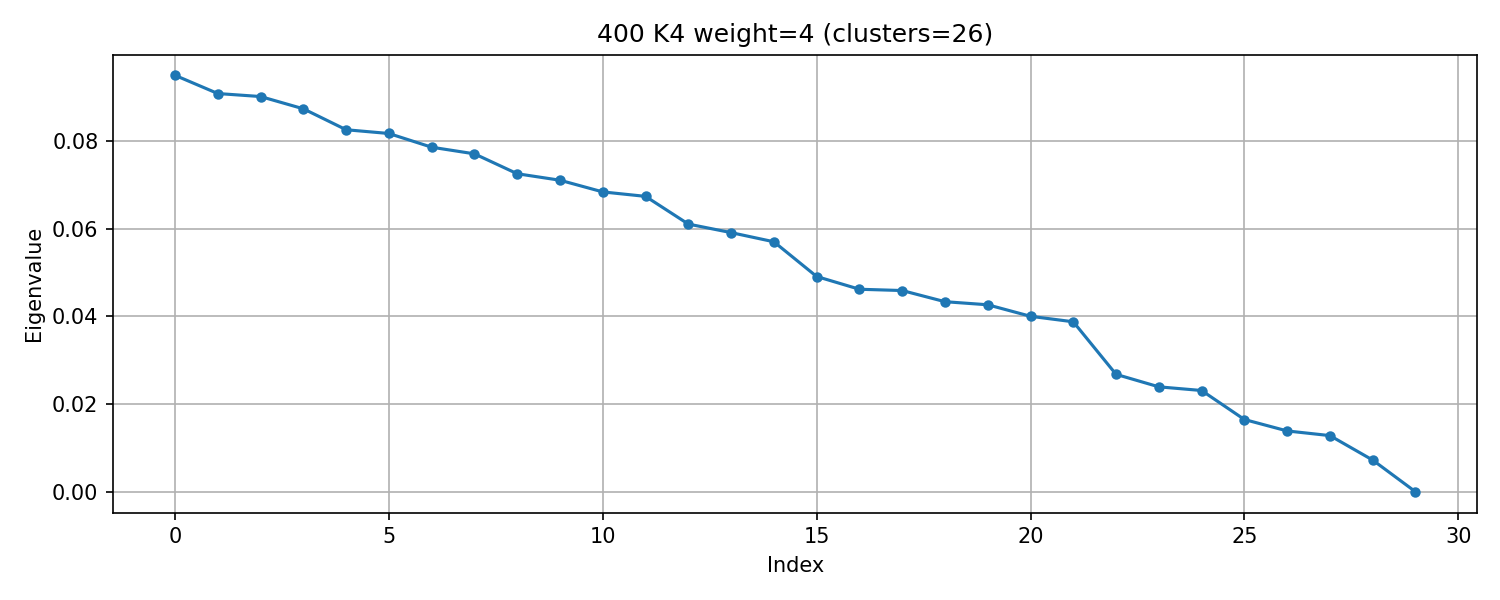
\includegraphics[width=0.45\textwidth]{figures/strong_L12_400_4.png}
\caption{Splitting of eigenvalues after adding $K_4$ anchors.}
\label{fig:triplet_anchored}
\end{figure}

\subsection{Black Hole Collapse ($3\to2$): Dimensional Unlocking}
Increasing the gravitational intensity at the center of a $L=8$ cubic grid causes the spectral dimension $d_s$ to drop from $\approx2.65$ to $\approx2.41$ when the intensity exceeds a threshold ($\approx5.67$), as shown in Fig.~\ref{fig:bh_collapse}. This phase transition corresponds to the failure of strong anchoring and the collapse of 3D space back to a 2D holographic surface, providing qualitative support for the geometric origin of the black hole entropy area law. Code: \texttt{blackhole\_exp.py}.

\begin{figure}[H]
\centering
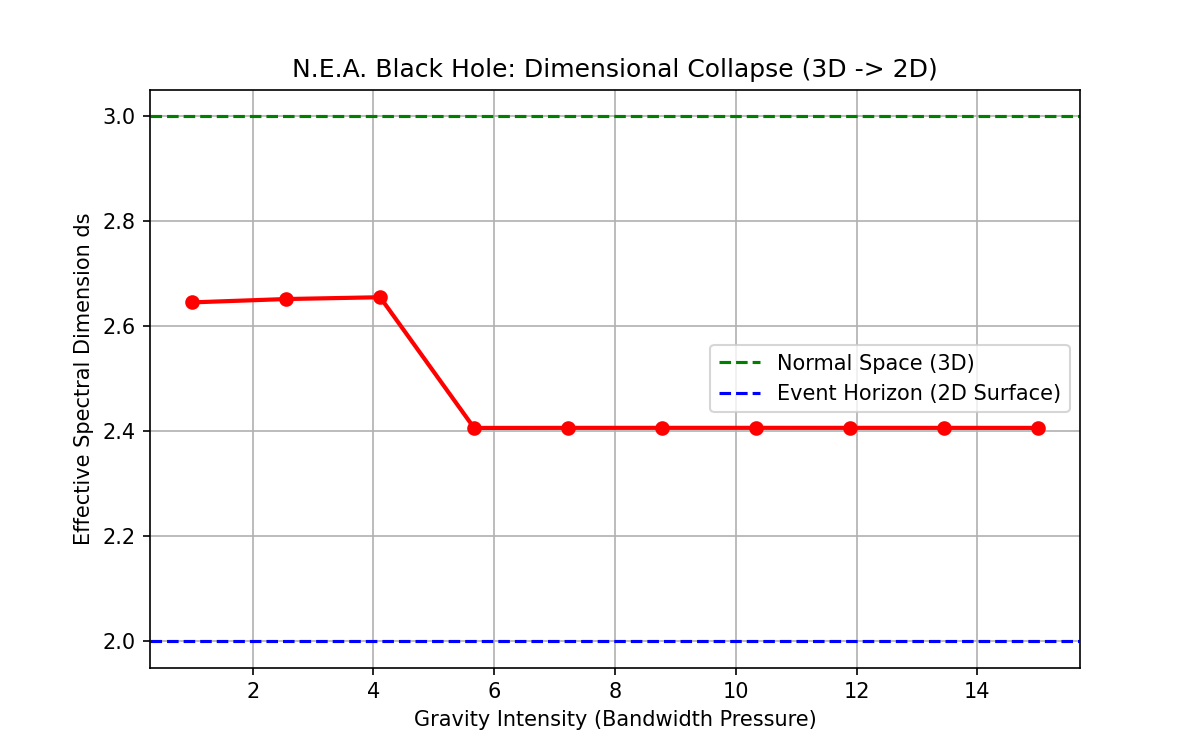
\includegraphics[width=0.6\textwidth]{figures/bh_collapse.png}
\caption{Black hole collapse: spectral dimension drops from 2.65 to 2.41.}
\label{fig:bh_collapse}
\end{figure}

\section{Discussion}
\subsection{The Possibility of Higher Dimensions}
Each dimensional increase demands a geometric rise in bandwidth cost to maintain connectivity. Under the total enthalpy (bandwidth) of our universe, the 3D stretching and 4D anchoring represent the most efficient equilibrium. Constructing a macroscopic 4D space (i.e., stretching a 3D volume to a 4D hypersolid) would likely exceed the node bandwidth limit, causing irreversible spatial anemia. However, this does not preclude the existence of higher dimensions:
\begin{itemize}
    \item In other universes with larger total bandwidth, dimensions beyond 3 may be stable.
    \item In our universe, extra dimensions could be ``frozen'' or compactified: they exist geometrically but cannot be macroscopically excited due to high bandwidth costs, appearing only as quantum fluctuations or compactified dimensions as in string theory.
\end{itemize}
Thus, the N.E.A. framework does not deny higher dimensions but provides a bandwidth-based criterion for their viability.

\subsection{On the Anti-universe and Dimensional Symmetry}
In the N.E.A. framework, the dimensional ladder follows an alternating “zig‑zag” pattern: expansion (weak force) followed by anchoring (electromagnetic force), then expansion (gravity) followed by anchoring (strong force). This alternating structure has an important consequence: it satisfies Noetherian conservation internally without requiring an external compensating partner. Each expansion that adds degrees of freedom is later constrained by an anchoring step, so the total enthalpy can remain constant.

If one instead assumed a purely monotonic ladder (all forces acting as pure expansions with no alternating anchors), then each dimensional increase would monotonically raise the total degrees of freedom, violating conservation. To compensate, one might be forced to postulate an anti‑universe with negative dimensions ($-1,-2,-3,-4$) and opposite force polarities, such that the conserved quantities of the two universes sum to zero. Such an anti‑universe would be a logical possibility under CPT symmetry.

However, within the N.E.A. framework we find no numerical evidence or theoretical necessity for an anti‑universe:
\begin{itemize}
    \item Our graph‑theoretic models (adjacency matrices, Laplacians, spectral dimensions) are built on non‑negative edge weights, yielding non‑negative eigenvalues. Constructing negative dimensions would require negative edge weights or negative eigenvalues, which are physically meaningless here (e.g., they would lead to imaginary internal clock frequencies).
    \item Even if one attempted to take a continuum limit, the spectral dimension is a real number defined through the asymptotic behavior of the heat kernel; it is not the value of an analytic function that can be continued to negative arguments. There is no analytic continuation path from positive dimensions ($1,2,3,4$) to negative ones ($-1,-2,-3,-4$).
    \item Hence, while an anti‑universe remains a speculative symmetry conjecture, it lies outside the computational and mathematical tools of the present framework. The framework neither predicts nor excludes it – it simply cannot be tested with our current methods.
\end{itemize}
Therefore, the zig‑zag ladder is self‑consistent and conserves the total enthalpy without invoking an anti‑universe. The question of a possible anti‑universe is left as an open problem for future theoretical or experimental exploration.

\section{Open Questions and Limitations}
\begin{itemize}
    \item The $0\to1$ corner (birth of causality) remains an abyss whose computational origin is unknown.
    \item The finite-size scaling of the 2D Weaver shows $d_s$ increasing slowly; the convergence limit is not yet determined, and larger-scale simulations are required.
    \item The $K_4$ anchoring model is heuristic; a rigorous derivation from $K_4$ to the $SU(3)$ gauge group is required.
    \item Quantitative reproduction of the intergenerational mass ratio $m_s/m_d\approx20$ has not yet been achieved.
    \item All numerical simulations are limited to moderate scales ($N\leq10000$); extrapolation to the continuum limit has limited reliability.
    \item The possible existence of an anti‑universe (a CPT‑mirrored branch with negative dimensions) cannot be addressed by the current framework, as it would require negative edge weights or analytic continuation beyond the spectral dimension’s definition.
\end{itemize}

\section{Conclusion}
We have presented a heuristic unified perspective, ``topological genesis of dimensions,'' supported by preliminary numerical experiments and astronomical observations. The 1D chain spectral dimension, finite-size scaling of 2D weaving, galaxy rotation curve blind test, triple degeneracy in 3D grids, and black hole dimensional collapse are all consistent with the $0$-$1$-$2$-$3$-$4$ zig-zag ladder. Despite open issues and the abyss at $0\to1$, this work provides a new testable framework for understanding fundamental forces as anchors of dimensionality. The validity of the ladder awaits stricter mathematical proofs and larger-scale simulations.

\section*{Data and Code Availability}
All numerical codes are open-sourced at \url{https://github.com/hzhangy/neaduality}. Gravitational observational data (SPARC fits, blind test) are from the independent repository \url{https://github.com/hzhangy/nea2gravity} (Paper IV).

\section*{Acknowledgments}
The authors thank the AI collaboration team for intensive computational support.

\begin{thebibliography}{99}
\bibitem{sparc} Lelli, F., McGaugh, S. S., \& Schombert, J. M. (2016). SPARC: Mass Models for 175 Disk Galaxies with Spitzer Photometry and Accurate Rotation Curves. \textit{AJ}, 152, 157.
\bibitem{book} Zhang, Y. (2024). \textit{Being is Time}. Chinese edition.
\bibitem{rindler} Jacobson, T. (1995). Thermodynamics of Spacetime: The Einstein Equation of State. \textit{Phys. Rev. Lett.}, 75, 1260.
\bibitem{verlinde} Verlinde, E. (2011). On the Origin of Gravity and the Laws of Newton. \textit{JHEP}, 1104, 029.
\bibitem{bombelli} Bombelli, L., et al. (1987). Space–time as a causal set. \textit{Phys. Rev. Lett.}, 59, 521.
\bibitem{ambjorn} Ambjørn, J., Jurkiewicz, J., \& Loll, R. (2005). Reconstructing the Universe. \textit{Phys. Rev. D}, 72, 064014.
\bibitem{milgrom} Milgrom, M. (1983). A modification of the Newtonian dynamics as a possible alternative to the hidden mass hypothesis. \textit{ApJ}, 270, 365.
\end{thebibliography}

\end{document}